\documentclass[11pt, a4paper]{article}
\usepackage{amsmath, amssymb}
\usepackage{booktabs}
\usepackage{tabularx}
\usepackage{minted}
\usepackage{tcolorbox}
\usepackage{graphicx}
\usepackage[utf8]{inputenc}
\usepackage[T1]{fontenc}
\usepackage{geometry}
\geometry{margin=1in}

% Custom commands and environments
\newcommand{\sta}{\textbf{\sffamily [CRITICAL / EXAM]\ }}

\newenvironment{important}
  {\begin{tcolorbox}[colback=blue!5!white, colframe=blue!75!black, arc=1mm, boxrule=1pt]}
  {\end{tcolorbox}}


\begin{document}
% Lecture Notes: Multiple Sequence Alignment (Part 1)

\section{Introduction to Evolutionary Trees and Multiple Sequences}

Evolutionary biology relies heavily on computational approaches to trace the relationships between species over time. While pairwise sequence alignment is foundational for comparing two sequences, complex biological studies—such as reconstructing Charles Darwin's conceptual "tree of life"—require us to evaluate many sequences simultaneously. 

By analyzing the genomic or proteomic similarities among different organisms, we can infer their evolutionary histories. For example, creating evolutionary trees of Madagascan reptiles or tracking the divergence of SARS-CoV-2 variants (like Alpha, Beta, or Omicron) depends on effectively aligning and comparing numerous genetic sequences at once.

% [IMAGE: Evolutionary tree of Madagascan reptiles based on similarities in the COI gene, showcasing how species branch out based on sequence similarity.]
% [IMAGE: The Tree of Life Explorer diagram, showing major branches of living species and some extinct ones, like Dionaea.]
% [IMAGE: SARS-CoV-2 Evolutionary Tree Data as of March 15, 2022, tracing the emergence and divergence of different viral variants over time.]

\subsection{The Principle of Parsimony in Evolution}

When determining how sequences evolved from a common ancestor, we rely on the principle of parsimony. This principle suggests that the most likely evolutionary path is the one requiring the fewest changes. 

\begin{important}
  \textbf{Evolutionary Parsimony}: A principle stating that when multiple evolutionary paths are possible, the most probable history is the one with the fewest mutations, insertions, or deletions.
\end{important}

Applying parsimony to sequence alignment yields the following expectations:
\begin{itemize}
    \item \textbf{Match:} If two species share the same nucleotide or amino acid at a position, it is highly likely that their common ancestor also had this character and nothing changed during evolution.
    \item \textbf{Mismatch:} If there is a disagreement, it is most likely that only one of the two sequences mutated from the ancestral state, rather than both independently mutating.
    \item \textbf{Gap:} An insertion or deletion occurred in one of the lineages with respect to the common ancestor.
\end{itemize}

\subsection{From Pairwise to Multiple Sequence Alignment}

Until now, computational techniques like global alignment, local alignment, and read mapping strictly compared two sequences at a time. However, a \textbf{Multiple Sequence Alignment (MSA)} analyzes more than two sequences simultaneously. This provides a more generalized view of relationships and helps resolve ambiguities that pairwise alignments cannot handle.

\textbf{Example:} Resolving alignment ambiguities with MSA.
Suppose we are aligning the English word "SUGAR" and the French word "SUCRE" (which share a common linguistic ancestor).
\begin{itemize}
    \item \textbf{Alternative 1 (High gaps):} \texttt{S U G A R -} aligned with \texttt{S U C - R E}
    \item \textbf{Alternative 2 (No gaps, high mismatch):} \texttt{S U G A R} aligned with \texttt{S U C R E}
\end{itemize}
In a strict pairwise comparison with heavy gap penalties, Alternative 2 might score better. However, if we introduce other languages into an MSA (e.g., \texttt{S A K A R I}, \texttt{Z U K E R}), we observe that the letter "R" is conserved across almost all sequences at the same relative position. This evolutionary context indicates that Alternative 1 is biologically correct, as aligning the "R"s across all sequences justifies the insertion of gaps.

\sta MSA allows us to extrapolate better pairwise relationships by leveraging the shared evolutionary context of the entire sequence set.

\section{Formalizing Multiple Sequence Alignment}

To compute an MSA, we must formally define it. The goal is to insert gaps into a set of sequences such that they all reach the exact same length, allowing them to be stacked and compared column by column.

\begin{important}
  \textbf{Multiple Sequence Alignment (MSA)}: Given $k$ strings $S_1, S_2, \dots S_k$ over an alphabet $\Sigma$, a multiple alignment is a set of $k$ strings $S'_1, S'_2, \dots S'_k$ over the extended alphabet $\Sigma' = \Sigma \cup \{-\}$ such that:
  \begin{itemize}
      \item $|S'_1| = |S'_2| = \dots = |S'_k|$ (all sequences have the same length after alignment).
      \item For all $i \in \{1 \dots k\}$, $S'_i$ is obtained from $S_i$ solely by inserting gaps (\texttt{-}).
  \end{itemize}
\end{important}

% [IMAGE: Alignment of ArgR binding sites in Pseudomonas aeruginosa, showing how MSA is used not just for different species, but to compare repeated elements (like binding sites) within a single genome.]

\subsection{Sum of Pairs (SP) Score}

To determine the optimal placement of gaps, we need a scoring function to maximize (or a distance function to minimize). The most common formalization is the Sum of Pairs score.

\begin{important}
  \textbf{Sum of Pairs (SP) Score}: The overall score of an MSA computed by summing the pairwise alignment scores for every possible pair of sequences in the alignment.
  \[
  SP = \sum_{i=1}^{k-1} \sum_{j=i+1}^k a(S_i, S_j)
  \]
  where $a(S_i, S_j)$ is the alignment score between sequence $i$ and sequence $j$.
\end{important}

Our objective becomes an optimization problem: find the multiple alignment that maximizes the SP score.

\section{Exact Solutions via Dynamic Programming}

Just as we used a 2D matrix for aligning two sequences, we can generalize dynamic programming to $k$ sequences.
\begin{itemize}
    \item For $k=2$, we fill a 2D matrix.
    \item For $k=3$, we fill a 3D structure (a cube).
    \item For $k>3$, we use a $k$-dimensional structure (a hypercube or hyperlattice).
\end{itemize}

The principle remains identical: to fill a cell, we evaluate the scores of all immediate neighboring cells, add the corresponding transition score, and pick the maximum. The final cell in the hyperlattice contains the global optimal MSA score.

\subsection{Neighboring Cells and Transitions}

The complexity of the dynamic programming approach scales rapidly due to the number of neighbors.
\begin{itemize}
    \item For $k=2$, a cell has 3 neighbors (top, left, diagonal).
    \item For $k=3$, a cell has 7 neighbors (faces, edges, and the main diagonal of the unit cube).
    \item For $k$ sequences, a cell has $2^k - 1$ neighbors.
\end{itemize}

When calculating the transition score $\delta(x, y, z)$ to move into a new cell for $k=3$, we decompose the column into pairwise comparisons. 

\textbf{Example:} Calculating a column score.
Consider adding a column with a match and mismatches: \texttt{C}, \texttt{G}, \texttt{G}. 
\[
\text{Column Score} = s(C,G) + s(C,G) + s(G,G) = \text{Match} + 2 \cdot \text{Mismatch}
\]
Consider adding a column with one nucleotide and two gaps: \texttt{A}, \texttt{-}, \texttt{-}.
\[
\text{Column Score} = s(A,-) + s(A,-) + s(-,-) = 2 \cdot \text{GapPenalty}
\]
\sta Notice that $s(-,-) = 0$. Aligning two gaps does not change the biological meaning of the alignment, as we could arbitrarily insert columns of purely gaps without affecting the sequence relationships. Thus, it contributes exactly zero to the score.

\subsection{Complexity and NP-Hardness}

Assume we have $k$ sequences, each of length $n$.
\begin{itemize}
    \item \textbf{Space Complexity:} The hyperlattice requires $(n+1)^k$ cells, resulting in $O(n^k)$ space.
    \item \textbf{Time Complexity:} Filling each cell requires checking $2^k - 1$ neighbors, resulting in $O(2^k n^k)$ time.
\end{itemize}

Because $k$ is an input variable (the number of sequences), the space and time scale exponentially. 

\begin{important}
  \textbf{Theorem}: The Multiple Sequence Alignment problem is \textbf{NP-hard} for any non-trivial scoring function. It cannot be solved in polynomial time (unless P=NP). In practice, optimal hypercube DP is unfeasible for more than 4 to 6 sequences.
\end{important}

\section{Approximation Algorithms: The Center Star Algorithm}

Since exact calculation is intractable for realistic datasets (e.g., 20 sequences of length 200), we must rely on heuristics and approximation algorithms. A good approximation algorithm runs in polynomial time and guarantees that its solution is within a certain ratio ($\varepsilon$) of the true optimal solution.

The \textbf{Center Star Algorithm} is a progressive alignment heuristic. It operates on the intuition that highly similar sequences require fewer gaps to align, reducing the likelihood of placing a gap in the wrong position.

\begin{minted}{python}
# [pseudocode]
def center_star(sequences):
    best_sp_score = -infinity
    center_seq = None
    
    # Step 1: Compute all pairwise alignments
    for S_i in sequences:
        current_sp = 0
        for S_j in sequences:
            if S_i != S_j:
                current_sp += align(S_i, S_j).score
                
        # Step 2: Choose the center string
        if current_sp > best_sp_score:
            best_sp_score = current_sp
            center_seq = S_i

    # Steps 3 & 4: Build the final alignment progressively
    msa = initialize_alignment(center_seq)
    for seq in sequences:
        if seq != center_seq:
            # Add sequence, expanding gaps across the entire MSA
            msa = progressive_merge(msa, align(center_seq, seq)) 

    return msa
\end{minted}

The code above demonstrates the Center Star methodology. First, it iteratively compares every sequence against all others to find the "center of the star" — the sequence with the highest total similarity. Next, it builds the final MSA by merging the remaining sequences onto the center one-by-one. A crucial mechanism here is that if merging a new sequence requires inserting a gap into the center sequence, that gap is also inserted into all previously aligned sequences to maintain their relative alignment columns.

\textbf{Example:} Walkthrough of Center Star Gap Expansion.
\begin{enumerate}
    \item Pairwise alignments identify \texttt{S2} as the center string.
    \item We align \texttt{S1} to \texttt{S2}. The MSA currently has two rows.
    \item We align \texttt{S3} to the MSA. Suppose the pairwise alignment of \texttt{S3} to \texttt{S2} dictates that a gap must be placed in \texttt{S2}.
    \item We place the gap in \texttt{S2}, but we \textit{must} also insert a gap in the exact same column for \texttt{S1} to ensure \texttt{S1} and \texttt{S2} remain properly aligned relative to each other.
    \item We continue this process for all sequences. The order in which sequences are added to the center does not change the final alignment.
\end{enumerate}

\subsection{Complexity and Approximability of Center Star}

\begin{itemize}
    \item \textbf{Pairwise Alignments (Step 1):} Computing $O(k^2)$ pairwise alignments of length $n$ takes $O(k^2 n^2)$ time.
    \item \textbf{Merging (Steps 2-3):} Takes $O(k n)$ time.
    \item \textbf{Overall Complexity:} $O(k^2 n^2)$ time and space.
\end{itemize}

\sta \textbf{Practical Optimization:} If the pairwise alignments are executed sequentially, we can discard each DP matrix after use, reducing space complexity to $O(n^2)$. If executed in parallel across multiple cores, wall-clock time can be reduced to $O(n^2)$.

\begin{important}
  \textbf{Approximation Guarantee ($\varepsilon = 2$)}: If the scoring metric represents a distance and satisfies the triangle inequality ($z \le x + y$), the Center Star algorithm guarantees a solution whose overall distance is at worst exactly twice the optimal distance ($\varepsilon = 2$).
\end{important}

\section{Biological Limitations and Phylogenetic Trees}

While mathematically efficient, the Center Star algorithm forces an artificial topology: it treats all sequences as having evolved directly from the "center" sequence. In reality, sequences evolve through branching lineages.

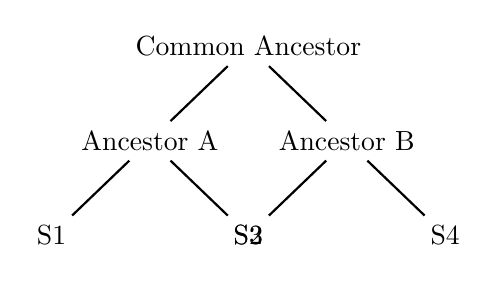
\begin{tikzpicture}[level distance=1.2cm, sibling distance=2.5cm, thick]
  \node {Common Ancestor}
    child { node {Ancestor A}
      child { node {S1} }
      child { node {S2} }
    }
    child { node {Ancestor B}
      child { node {S3} }
      child { node {S4} }
    };
\end{tikzpicture}

If the true evolutionary history (phylogenetic tree) matches the diagram above, a biologically accurate progressive alignment should:
\begin{enumerate}
    \item Align the closest relatives first (S1 with S2, and S3 with S4).
    \item Merge the resulting sub-alignments together.
\end{enumerate}
This requires the ability to align a sequence to an existing alignment, or merge two existing alignments together. To achieve this, we use alignment profiles.

\section{Alignment Profiles and Weighted Dynamic Programming}

\begin{important}
  \textbf{Alignment Profile}: A compact, mathematical representation of a multiple sequence alignment. For each column, it stores the relative frequency of each symbol (including gaps). The frequencies in any single column always sum to 1.
\end{important}

\begin{table}[htpb]
\centering
\caption{Example of an alignment profile derived from 3 sequences over 9 columns.}
\begin{tabularx}{\textwidth}{l X X X X X X X X X}
\toprule
Symbol & 1 & 2 & 3 & 4 & 5 & 6 & 7 & 8 & 9 \\
\midrule
A & 2/3 & 0   & 0   & 0   & 0   & 0   & 2/3 & 0   & 0 \\
C & 0   & 1   & 1/3 & 0   & 1   & 0   & 0   & 1/3 & 0 \\
G & 1/3 & 0   & 0   & 1   & 0   & 1/3 & 1   & 0   & 2/3 \\
T & 0   & 0   & 0   & 0   & 0   & 0   & 0   & 0   & 0 \\
- & 0   & 0   & 2/3 & 0   & 0   & 2/3 & 0   & 1/3 & 0 \\
\bottomrule
\end{tabularx}
\end{table}

While profiles compactly represent MSAs, they lose specific sequence linkage information (e.g., in column 1, we know $2/3$ of the sequences have an 'A', but we no longer know exactly \textit{which} input sequences those are). 

\subsection{Weighted Dynamic Programming}

To align a new sequence $X = (x_1, \dots, x_n)$ to an existing profile $R$, we use a 2D dynamic programming matrix. The rows represent the sequence to be added, and the columns represent the profile.

We evaluate the score of matching a character $x$ with column $j$ using the weighted sum:
\[
P(x, j) = \sum_{c \in \Sigma} sim(x, c) \times R[c, j]
\]
where $sim(x,c)$ is the standard pairwise scoring matrix (match, mismatch, or gap penalty), and $R[c,j]$ is the profile frequency.

The dynamic programming recurrence relation for a cell $A[i,j]$ is:
\[
A[i,j] = \max \begin{cases}
  A[i - 1, j - 1] + P(x_i, j) & \text{(align } x_i \text{ to profile column } j \text{; diagonal move)} \\
  A[i - 1, j] + \text{gap penalty} & \text{(introduce gap into profile; top move)} \\
  A[i, j - 1] + P(\text{`--'}, j) & \text{(introduce gap into sequence } x \text{; left move)}
\end{cases}
\]

\textbf{Example:} Filling the DP matrix.
Assume a match score of $+1$, mismatch penalty of $-1$, and gap penalty of $-1$. We are at the first letter of our new string ($x_1 =$ `A') and comparing it to the first column of the profile ($j=1$, which has $2/3$ `A' and $1/3$ `G').
\begin{enumerate}
    \item \textbf{Diagonal Move (Match `A' to column 1):} 
    Score $= 0 + P(\text{`A'}, 1) = (1 \times \frac{2}{3}) + (-1 \times \frac{1}{3}) = \frac{1}{3}$.
    \item \textbf{Top Move (Gap in profile):}
    This means we map `A' against a 100\% gap column. We start at the previous gap penalty ($-1$) and add another full gap penalty ($-1$). Total $= -2$.
    \item \textbf{Left Move (Gap in string):}
    We map a gap (`-') against column 1. The score is $-1 + P(\text{`-'}, 1) = -1 + (-1 \times \frac{2}{3}) + (-1 \times \frac{1}{3}) = -2$.
\end{enumerate}
The maximum is the diagonal move ($\frac{1}{3}$), so we record that value and place a traceback pointer pointing diagonally.

\sta \textbf{Initialization Nuance}: When initializing the first row (adding gaps into the sequence being aligned), the gap penalty is weighted by the fraction of non-gap characters in the profile. If a profile column is already $2/3$ gaps, penalizing the alignment of a new gap against it is less severe, since gaps are already biologically expected at that position.

By repeating this weighted algorithm, we can progressively build highly accurate, biologically relevant alignments guided by a phylogenetic tree.

\subsection{Traceback and Profile Updating}

Once the dynamic programming matrix is completely filled using the weighted scoring rules, the overall optimal score for aligning the new sequence to the profile is found in the final cell (bottom-right). Just as in standard pairwise global alignment, we must perform a \textbf{traceback} to reconstruct the actual alignment.

\begin{enumerate}
    \item \textbf{Traceback Phase:} Starting from the final cell, we follow the pointers recorded during the matrix filling phase (diagonal, top, or left) back to the origin cell. This reconstructs the sequence of matches, mismatches, and gap insertions.
    \item \textbf{Profile Updating:} The reconstructed alignment tells us exactly how the new sequence maps to the existing columns of the profile (or where new gap columns must be inserted into the profile). We add the new string to the existing set of aligned sequences and \textit{recompute all frequencies} to create an updated alignment profile.
    \item \textbf{Iterative Addition:} This new, updated profile is then used as the column input for the dynamic programming matrix of the next sequence to be added.
\end{enumerate}

\sta \textbf{Crucial Advantage:} The primary advantage of this weighted profile method over the Center Star algorithm is that we no longer compare the new sequence to just a single "center" sequence. Instead, the profile forces the alignment to explicitly account for the biological variation of \textit{all} previously aligned sequences simultaneously.

\subsection{Profile-Profile Alignment}

The weighted dynamic programming approach is not restricted to aligning a single new sequence to a profile. To accurately follow a complex evolutionary tree (like merging an alignment of $S_1, S_2$ with an alignment of $S_3, S_4$), we must be able to align two profiles together.

\begin{important}
  \textbf{Profile-Profile Alignment}: The process of aligning two existing multiple sequence alignments to each other. Both the rows and the columns of the dynamic programming matrix represent alignment profiles rather than individual sequences.
\end{important}

To compute the cell scores for a profile-profile alignment, we use a \textbf{double-weighted} version of the scoring rule. Instead of comparing a single character $x$ to a profile column $j$, we compare the frequencies in profile column $i$ (from the first alignment) with the frequencies in profile column $j$ (from the second alignment), calculating the expected score across all possible pairs of characters weighted by their joint probabilities.

\section{Progressive Multiple Alignment and Guide Trees}

Algorithms that build a multiple sequence alignment step-by-step—either by adding sequences to a profile or by merging profiles together—are generally classified as \textbf{progressive alignment algorithms}. 

To execute a progressive alignment correctly, the algorithm must know the specific order of operations. Which two sequences should be aligned first? Which sequence or sub-alignment should be merged next?

\begin{important}
  \textbf{Guide Tree}: A tree structure (often a predicted phylogenetic tree) that dictates the pairing order for a progressive multiple sequence alignment. The closest leaves on the tree are aligned first, and the alignment progresses toward the root.
\end{important}

\subsection{The Circular Dependency Problem}

Using a guide tree to perform progressive alignment introduces a fundamental Catch-22 in computational biology:
\begin{itemize}
    \item To build an accurate \textbf{evolutionary (phylogenetic) tree}, we need a high-quality Multiple Sequence Alignment to identify conserved and divergent regions.
    \item To build a high-quality \textbf{Multiple Sequence Alignment} using progressive methods, we need a guide tree to tell us the correct evolutionary order of operations.
\end{itemize}

\sta \textbf{Resolution:} In practice, bioinformatics tools solve this circular dependency through a bootstrap approach. Before proceeding with the heavy computational work of weighted profile alignment, the algorithm first \textit{predicts} an approximate guide tree. It usually does this by rapidly calculating rough pairwise distances (often using fast heuristics rather than full dynamic programming) to establish a baseline topology. Once this rough tree is predicted, it serves as the guide tree to drive the rigorous progressive multiple sequence alignment.

\end{document}